\documentclass[UTF8]{ctexart}
\usepackage{graphicx}
\usepackage{amsmath}
\usepackage{bibentry,natbib}
\usepackage{fancyhdr}

\title{Latent Dirichlet Allocation}
\author{BrightHush}
\date{\today}

\begin{document}
\maketitle
\tableofcontents

\pagestyle{fancy}
\cfoot{\thepage}

\newcommand{\figref}[1]{\figurename~\ref{#1}}
%\begin{figure}[h!]
%    \centering     
%    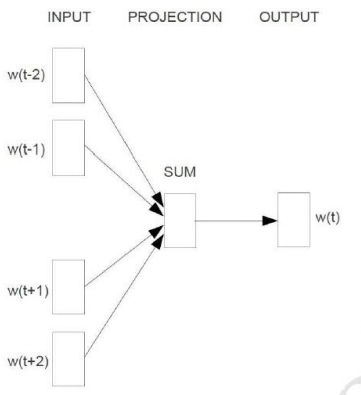
\includegraphics[width=0.5\textwidth]{cbow}   
%    \caption{\label{Fig:CBOW}CBOW Architecture} 
%\end{figure}

\section{LDA with Gibbs Sampling}

\subsection{Basic Distribution Knowledge}
\textbf{Gamma function} 阶乘的扩展,如果n是整数,那么:
\begin{align}
\Gamma(n) = (n-1)!
\end{align}
gamma function 对负整数和0没有定义之外,对于实部为整数的复数,其定义为一个积分:
\begin{align}
\Gamma(t) = \int_{0}^{\infty}x^{t-1}e^{-x}dx
\end{align}
\par
\textbf{Dirichlet dsistribution} 有K($K \geq 2$)个参数,表示为$\alpha = (\alpha_1, \alpha_2, ..., \alpha_K)$,
其中$\alpha_i > 0$,有K个变量分别表示为($x_1, x_2, ..., x_K$),其中$x_i \in \left[0, 1 \right]$,
并且$\sum_{i=1}^K x_i = 1$。
其概率密度函数可以表示为:
\begin{align}
f(x_1, ..., x_K; \alpha) = \frac{1}{B(\alpha)} \Pi_{i=1}^K x_{i}^{\alpha_i - 1}
\\
\sum_{i=1}^K x_i = 1
\\
B(\alpha) = \frac{\Pi_{k=1}^K \Gamma(\alpha_i)}{\Gamma(\sum_{k=1}^K \alpha_i)}
\end{align}
为了和 Parameter estimation for text analysis 一文中的记号表示一致,在下面的笔记中,$B(\alpha)$统一用$\Delta(\alpha)$来表示。
其中各变量的期望和最大值可以表示如下:
\begin{align}
E\left[ x_i \right] = \frac{\alpha_i}{\sum_{k=1}^K \alpha_k}
\\
x_i = \frac{\alpha_i - 1}{\sum_{k=1}^K \alpha_i - K} \ \ \ Mode
\end{align}
Dirichlet 分布的边缘分布是Beta分布,可以表示如下:
\begin{align}
x_i \sim Beta(\alpha_i, \sum_{k=1}^K \alpha_k - \alpha_i)
\end{align}
Dirichlet分布有一个特殊的情况,就是\textbf{Symmetric Dirichlet Distribution},所谓对称Dirichlet分布
就是参数$\alpha$的各个分量相同,也就是各个$\alpha_i$具有相同的值。通常情况下,如果先验知识中并没有关于一个分量
比另外一个分量更重要的信息,那么 Symmetric Dirichlet Distribution 通常被作为先验分布。
Symmetric Dirichlet Distribution
可以表示如下:
\begin{align}
f(x_1, \cdots, x_K; \alpha) = \frac{\Gamma(K\alpha)}{\Gamma(\alpha)^K} \Pi_{k=1}^K x_k^{\alpha-1}
\end{align}

\subsection{Parameters Table}
\begin{itemize}
\item[$p(w=t|z=k)$]: a multinomial distribution over terms that corresponding 
one of the latent topics z=k.
\item[$p(t|z=k)=\vec{\varphi_k}$]: term distribution for each topic k.
\item[$p(z|d=m)=\vec{\vartheta_m}$]: topic distribution for each document m.
\item[$\underline{\phi}=\left( \vec{\varphi_k} \right) _{k=1}^K$]: parameter set.
\item[$\underline{\theta}=\left( \vec{\vartheta_m}\right)_{m=1}^M$]: parameter set.
\item[$M$]: number of document to generate (constant scalar).
\item[$K$]: number of topics (constant scalar).
\item[$V$]: number of terms $t$ in vocabulary (constant scalar).
\item[$\vec{\alpha}$]: hyper parameter of Dirichlet distribution which is prior distribution of
 doc-topic multinomial distribution.
\item[$\vec{\beta}$]: hyper parameter of Dirichlet distribution which is prior of topic-term 
multinomial distribution.
\item[$N_m$]: length of document m.
\item[$z_{m,n}$]: topic indicator for the nth word in document m.
\item[$w_{m,n}$]: term indicator for the nth word in document m.
\end{itemize}

\subsection{Mixture modelling}
LDA是一种混合模型,其使用一组子分布加权来建模观察到的数据,其实也就是使用主题分布作为分量,
那么每个词的概率可以表示为:
\begin{align}
p(t=w) = \sum_{k=1}^K p(t=w|z=k)p(z=k|), \ \sum_{k=1}^K p(z=k) = 1
\end{align}
但是LDA中的主题分布并不是全局一样的,而是基于每一篇文档主题分布情况是不同的,于是在LDA中
有两组目标需要推断(1)主题k下的词分布$p(t|z=k)=\vec{\varphi}_k$和(2)文档m下的
主题分布$p(z|d=m)=\vec{\vartheta}_m$。

\subsection{Generative model}
为了获得推断策略,LDA生成模型的过程可以被理解为如下内容:对于每一篇文档,首先生成主题分布
$\vec{\vartheta}_m$,对于文档中的每个词,根据$\vec{\vartheta}_m$各主题占比分布对每个
词选择一个主题,用$z_{m,n}$表示,那么根据这个词所在主题的$\vec{\varphi}_{z_{m,n}}$来
生成这个词。需要注意的是$\vec{\varphi}_k$在整个语料中只会生成一次。

\subsection{Likelihoods}
对于整个语料集,如果每一个词都被赋予了主题标记$z_{m,n}$,那么一篇文档的似然可以表示为:
\begin{align}
L(\vec{w}_m, \vec{z}_m, \vec{\vartheta}_m, \vec{\phi}) = \Pi_{n=1}^{N_m}
p(w_{m,n}|\vec{\varphi}_{z_{m,n}}) p(z_{m,n}|\vec{\vartheta}_m) p(\vec{\vartheta}_m|\vec{\alpha}) p(\phi|\vec{\beta})
\end{align}
\par
对于一篇文档中的一个词,其产生的概率可以表示为(57)(\ref{57}):
\begin{align}
\label{57}
p(w_{m,n}=t|\vec{\vartheta}_m, \underline{\phi}) = \sum_{k=1}^K
p(w_{m,n}=t|\vec{\varphi}_k) \cdot p(z_{m,n}=k|\vec{\vartheta}_m)
\end{align}
对于语料$W=(\vec{w}_m)_{m=1}^M$,每篇文档的生成是独立的,每篇文档中的每个词生成过程也是独立的,
所以语料的似然可以表示为(58)(\ref{58}):
\begin{align}
\label{58}
L = p(W|\underline{\theta}, \underline{\phi}) = \Pi_{m=1}^M 
p(\vec{w}_m|\vec{\vartheta}_m, \underline{\phi}) = \Pi_{m=1}^M \Pi_{n=1}^{N_m}
p(w_{m,n}|\vec{\vartheta}_m, \underline{\phi})
\end{align}


\subsection{Inference via Gibbs Sampling}
对于包含隐含变量$\vec{z}$,其后验概率$p(\vec{z}|\vec{x})$通常是比较需要的分布,
对于这样包含隐含变量模型的通用Gibbs sampler的公式可以表示如下(60)(\ref{60})公式所示:
\begin{align}
\label{60}
p(z_i|\vec{z}_{\neg i}, \vec{x}) &= \frac{p(\vec{z}, \vec{x})}{p(\vec{z_{\neg i}}, \vec{x})}
\\
&= \frac{p(\vec{z},\vec{x})}{\int_{Z}p(\vec{z}, \vec{x})dz_i}
\end{align}
其中分母如果是对离散变量,那么可以改为对离散变量求和。按照Gibbs Sampling的思路,不断根据分量的条件概率进行
采样,假设我们每次采样得到的样本为$\tilde{\vec{z_r}}, r \in [1, R]$,如果采样次数足够多的话,那么
隐含变量的后验概率可以表示为(61)(\ref{61}):
\begin{align}
\label{61}
p(\vec{z}|\vec{x}) \approx \frac{1}{R}\sum_{r=1}^R \delta(\vec{z} - \vec{z_r})
\end{align}
其中$\delta(\vec{u}) = {1 \ if \ \vec{u}=0;\  0 \  otherwise}$。

\subsection{The collapsed LDA Gibbs Sampler}
为了设计出LDA的Gibbs Sampler,我们使用上面提到的隐含变量方法,在我们的模型中,隐含变量是$z_{m,n}$,也就是
语料中词$w_{m,n}$相对应的主题。通过对$z_{m,n}\ and \ w_{m,n}$进行统计,可以得到其他参数的情况。
\par
现在我们推断的目标是$p(\vec{z}|\vec{w})$,也就是每个词对应的主题情况,如(62)(\ref{62})所示:
\begin{align}
\label{62}
p(\vec{z}|\vec{w}) = \frac{p(\vec{z},\vec{w})}{p(\vec{w})} 
= \frac{\Pi_{i=1}^W p(z_i, w_i)}{\Pi_{i=1}^W\sum_{k=1}^Kp(z_i=k,w_i)}
\end{align}
由于上式中的分母计算量比较大,那么这个时候Gibbs Sampling派上用场了,为了仿真$p(\vec{z}|\vec{w})$,我们根据
$p(z_i|\vec{z_{\neg i}}, \vec{w})$进行Markov Chain进行Gibbs Sampling。根据公式(60)(\ref{60}),
需要知道联合分布概率。
\par
\emph{\textbf{Joint Distribution.}} LDA中的联合分布可以分解为(63)(\ref{63}):
\begin{align}
\label{63}
p(\vec{w}, \vec{z} | \vec{\alpha}, \vec{\beta}) &=
p(\vec{w}|\vec{z},\vec{\beta}) p(\vec{z}|\vec{\alpha})
\end{align}
等式(\ref{63})右边第一项可以表示为(64)(\ref{64}):
\begin{align}
\label{64}
p(\vec{w} | \vec{z}, \underline{\phi}) = \Pi_{i=1}^W p(w_i|z_i) 
= \Pi_{i=1}^W \varphi_{z_i, w_i}
\end{align}
上式是表示每个词从独立的多项分布中产生,我们可以将上面的乘积拆成两项,第一项按照主题乘积,第二项按照词汇表
乘积,于是可以表示为(65)(\ref{65}):
\begin{align}
\label{65}
p(\vec{w} | \vec{z}, \underline{\phi}) = 
\Pi_{k=1}^K \Pi_{i:\ z_i=k} p(w_i=t|z_i=k) =
\Pi_{k=1}^K \Pi_{t=1}^V \varphi_{k,t}^{n_k^{(t)}}
\end{align}
其中$n_k^{(t)}$表示词t在主题k下出现的次数。\\
上式表示的是在一组确定的$\phi$参数下词出现的条件概率,我们知道$\phi$中的参数是有Dirichlet先验的,
因此将上式对$\phi$进行积分或者累加,那么就能求得在超参$\beta$下的词条件概率:
\begin{align}
p(\vec{w}|\vec{z}, \vec{\beta}) &= \int 
p(\vec{w}|\vec{z}, \underline{\phi}) p(\underline{\phi}|\vec{\beta}) d\underline{\phi}
\\
&= \Pi_{z=1}^K \frac{\triangle(\vec{n_z}+\vec{\beta})}{\triangle(\vec{\beta})},
\vec{n_z}=\left( n_z^{(t)} \right)_{t=1}^V
\end{align}
\par
同理按照$p(\vec{w}|\vec{z}, \vec{\beta})$的推导,可以对$p(\vec{z}|\alpha)$进行类似的推导。
\begin{align}
p(\vec{z}|\theta) &= \Pi_{i=1}^W p(z_i|d_i)
\\
&= \Pi_{m=1}^M\Pi_{k=1}^K p(z_k=1|d_i=m)
\\
&= \Pi_{m=1}^M\Pi_{k=1}^K \vartheta_{m,k}^{n_m^{(k)}}
\end{align}
其中$d_i$表示词i对应的文档,$n_m^{(k)}$表示在文档m中,topic k出现的次数。上式对$\theta$进行
积分,可以得到:
\begin{align}
p(\vec{z}|\vec{\alpha}) &= \int p(\vec{z}|\underline{\theta}) p(\underline{\theta}|\vec{\alpha}) 
d\underline{\theta}
\\
&= \Pi_{m=1}^M \frac{\triangle(\vec{n_m}+\vec{\alpha})}{\triangle(\vec{\alpha})},
\vec{n_m}=\left( n_m^{(k)}\right)_{k=1}^K
\end{align}
于是可以得到主题和词的联合分部表示为:
\begin{align}
p(\vec{w}, \vec{z} | \vec{\alpha}, \vec{\beta}) = 
\Pi_{z=1}^K \frac{\triangle(\vec{n_z}+\vec{\beta})}{\triangle(\vec{\beta})}
\Pi_{m=1}^M \frac{\triangle(\vec{n_m}+\vec{\alpha})}{\triangle(\vec{\alpha})}
\end{align}
\par
\textbf{\emph{Full Conditional.}}根据联合概率分布,对于一个词$i=(m,n)$我们可以得到其条件概率,
也就是Gibbs Sampler采样一个隐含变量的条件概率,如式子(74,78)(\ref{74},\ref{78}):
\begin{align}
\label{74}
p(z_i=k|\vec{z_{\neg i}}, \vec{w}) = \frac{p(\vec{w}, \vec{z})}{p(\vec{w}, \vec{z}_{\neg i})}
= \frac{p(\vec{w}|\vec{z})}{p(\vec{w}_{\neg i}|\vec{z}_{\neg i})p(w_i)} \cdot 
\frac{p(\vec{z})}{p(\vec{z}_{\neg i})}
\\
\label{78}
\propto \frac{n_{k,\neg i}^{(t)} + \beta_t}{\sum_{t=1}^V n_{k, \neg i}^{(t)}+\beta_{t}}
(n_{m, \neg i}^{(k)} + \alpha_{k})
\end{align}
\par
\textbf{\emph{Multinomial Parameters.}}最终,我们需要求解多项分布的参数,这些参数用之前的参数集合$(\theta, \phi)$
表示。根据这些参数的定义,以及结合Dirichlet先验,根据贝叶斯公式,我们可以得到多项分布参数的后验估计,如
等式(79,80)(\ref{79},\ref{80})所示:
\begin{align}
\label{79}
p(\vec{\vartheta}_m|\vec{z}_m,\vec{\alpha}) &=
\frac{p(\vec{z}_m|\vec{\vartheta}_m)p(\vec{\vartheta}_m|\vec{\alpha})}{p(\vec{z}_m|\vec{\alpha})}
\\
&= \frac{p(\vec{z}_m|\vec{\vartheta}_m)p(\vec{\vartheta}_m|\vec{\alpha})}
{\int p(\vec{z}_m|\vec{\vartheta}_m)p(\vec{\vartheta}_m|\vec{\alpha}) d\vec{\vartheta}_m}
\\
&= \frac{\Pi_{k=1}^K \vartheta_{m,k}^{n_m^{(k)}} \frac{1}
{\Delta(\vec{\alpha})} \Pi_{k=1}^K \vartheta_{m,k}^{\alpha_k - 1} }
{\frac{\Delta(\vec{n}_m + \vec{\alpha})}{\Delta(\vec{\alpha})}}
\\
&= \frac{\Pi_{k=1}^K \vartheta_{m,k}^{n_m^{(k)} + \alpha_k - 1}}{\Delta(\vec{n}_m + \vec{\alpha})}
\\
&= \frac{1}{Z_{\vartheta _m}} \Pi_{n=1}^{N_m}
p(z_{m,n}|\vec{\vartheta}_m) \cdot p(\vec{\vartheta}|\vec{\alpha}) 
\\
&= Dir(\vec{\vartheta}_m|\vec{n}_m+\vec{\alpha})
\\
\label{80}
p(\vec{\varphi}_k|\vec{z},\vec{w}, \vec{\beta}) &= \frac{1}{Z_{\varphi_k}} \Pi_{i:z_i=k}
p(w_i|\vec{\varphi}_k) \cdot p(\vec{\varphi}_k|\vec{\beta}) 
\\
&= Dir(\vec{\varphi}_k | \vec{n}_k + \vec{\beta})
\end{align}
上式中$\vec{n}_m$表示第m篇文档中观察到的topic出现次数,$\vec{n}_k$则相应的表示在topic k中各词对应观察到的次数。\\
和(\ref{79})中的推导相似,(\ref{80})中表示的是主题下词的分布,由于$\varphi_k$是全局的,那么需要统计所有的词中,
主题被标记为k的词分布情况,就能得到该主题下词的分布了,如果用$w_k$表示主题k下各词出现情况,于是(\ref{80})的详细推导可以如下计算:
\begin{align}
p(\vec{\varphi}_k|\vec{w}_k, \vec{\beta}) &= 
\frac{p(\vec{w}_k|\vec{\varphi}_k)p(\vec{\varphi}_k|\vec{\beta})}{p(\vec{w}_k|\vec{\beta})}
\\ &=
\frac{\Pi_{t=1}^V \varphi_{k,t}^{n_k^{(t)}} \frac{1}{\Delta(\vec{\beta})} \Pi_{t=1}^V \varphi_{k,t}^{\beta_t -1}}
{\frac{\Delta(\vec{n}_k + \vec{\beta})}{\Delta(\vec{\beta})}}
\\
&= \frac{\Pi_{t=1}^V \varphi_{k,t}^{n_k^{(t)} + \beta_t -1}}{\Delta(\vec{n}_k+\vec{\beta})}
\\
&= Dir(\vec{\varphi}_k|\vec{n}_k+\vec{\beta})
\end{align}
根据Dirichlet Distribution的期望计算方法$<Dir(\vec{\alpha})> = \frac{\alpha_i}{\sum_i \alpha_i}$,那么根据(79,80)
(\ref{79}, \ref{80}),可以计算得到下面的结果:
\begin{align}
\label{81}
\varphi_{k,t} = \frac{n_k^{(t)}+\beta_t}{\sum_{t=1}^V n_k^{(t)}+\beta_t}
\\
\label{82}
\vartheta_{m,k} = \frac{n_m^{(k)}+\alpha_k}{\sum_{k=1}^K n_m^{(k)}+\alpha_k}
\end{align}


\section{References}
\begin{itemize}
\item[1] Parameter estimation for text anaylysis.\\
\url{http://www.52nlp.cn/unconstrained-optimization-one}.
\end{itemize}

\end{document}
